\chapter{Cahier des charges}


\section{Présentation et analyse du contexte}

Il existe de nombreux jeux de stratégie en temps réel, mais RTSoccer se déroule sur un terrain de foot que l’on peut considérer comme une arène, ce qui fait entrer le jeu dans la catégorie des MOBA (Multiplayer online battle arena). On y retrouve les mécaniques de ce type de jeu qui sont: le déplacement souris, l’utilisation de capacités, la gestion d’amélioration de son personnage ainsi que le multijoueur en ligne. Les MOBA les plus populaire sont League of Legends et Dota 2 (mais il en existe beaucoup d’autres) où les joueurs s’affrontent par équipe de 5 maximum et le but étant de détruire la base adverse.

RTSoocer est également un jeu de football mais qui ne suit pas les règles conventionnelles. Ainsi il est par exemple possible d’attaquer ses adversaire pour se frayer un chemin jusqu’a la cage adverse comme pour le jeu de Nintendo nommé Mario Smash Football où l’on contrôle une équipe de quatre joueurs dont un capitaine qui est le seul à pouvoir utiliser des capacités spéciales. Dans RTSoocer, le joueur contrôle un seul personnage avec lequel il peut utiliser certaines capacités pour attaquer ou défendre.

\section{Analyse des besoins fonctionnels}


\subsection{Le jeu et ses fonctionnalités}

RTSoccer se joue par match (ou partie) où deux équipes s’affrontent sur un terrain, le but étant de marquer des buts en faisant rentrer le ballon dans les cages de l’adversaire tout évitant d’en encaisser.
Chaque joueur incarne un personnage (un sportif) qu’il contrôle à l’aide de la souris et du clavier.

En cliquant avec la souris, le joueur indique la position où son avatar doit se rendre. Sur le terrain, les joueurs se dispute le ballon qu’ils peuvent récupérer en faisant passer leur personnage dessus (la récupération doit être automatique) au quel cas la balle reste “attaché” au personnage (si l’avatar se déplace, le ballon suit son mouvement en restant à ses pieds). Il est donc possible d’intercepter la balle en mouvement.

Avec le clavier, l'utilisateur peut déclencher une de ses capacités (au minimum 5 capacités différentes) qu’il oriente avec la souris (la capacité se déclenche dans le sens du curseur). Les capacités des sportifs sont les suivantes:\\

\begin{tabular}{|l|l|l|}
\hline
  Avec le ballon & Sans le ballon & Dans les 2 cas \\
\hline
  Charge & Frappe & Dash \\
  Vitesse & Frappe puissante  &  \\

\hline 
\end{tabular}

\vspace{.05in}
\begin{description}
  \item[Charge]: si la capacité touche un joueur, ce dernier est immobiliser pendant un certain moment et perd le contrôle de la balle.
  \item[Dash]: augmente la vitesse de déplacement du joueur pendant un laps de temps.
  \item[Frappe]: envoie le ballon dans la direction souhaité sur une certaine distance.
  \item[Frappe puissante]: c’est le même principe que “Frappe” mais le ballon part plus vite et la porté du tir est plus grande.
  \item[Vitesse]: permet de se “téléporter” rapidement à une position souhaitée (dans une limite distance).
\end{description}
\vspace{.05in}
%insertion figure
\begin{figure}[h!]
\centering
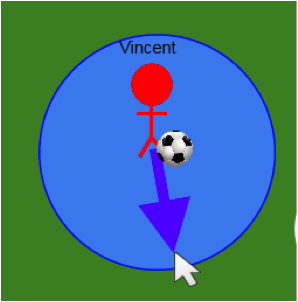
\includegraphics[scale=1]{fig1.png}
\caption{Exemple d'utilisation d'une capacité}
\end{figure}

Au cours de la partie, un joueur peut aussi charger les adversaires n’ayant pas la balle. Chacun de ces adversaires affectés rajoute au joueur un bonus de vitesse.

Le jeu est sans inscription, une fois sur le site, il suffit de rentrer son pseudonyme et on accède au gestionnaire des salles.

Au cours d'une partie, le joueur à la possibilité de dialoguer avec les membres de sa salle grâce au service de tchat disponible.


\subsection{Multijoueur}

Pour faire une partie de RTSoccer, les joueurs doivent au préalable rejoindre d’autres joueurs (qui sont leur coéquipiers et leurs adversaires) et choisir le temps que va durer la partie. 

Pour ce faire, le joueur peut créé une salle (ou en rejoindre une) où il définie les caractéristiques de la partie (nombre de joueur, durée de la partie). 
Ainsi les autres joueurs qui désire s’affronter sur le terrain peuvent rejoindre la salle et quand celle-ci est pleine, le créateur peut lancer la partie. 

Les utilisateurs peuvent consulter la liste des parties créées et les rejoindre.

%insertion figure
\begin{figure}[h!]
\centering
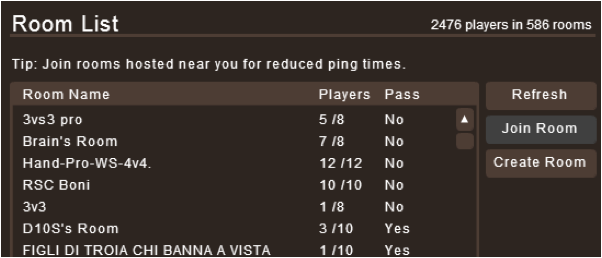
\includegraphics[scale=1]{fig2.png}
\caption{Exemple gestion de salle}
\end{figure}

\subsection{Diagramme de cas d'utilisation}

Ce diagramme présente l’ensemble des actions réalisables par le joueur lorsqu’il accède au site du jeu.

----------------
 A faire 
----------------

\section{Analyse des besoins non fonctionnels}

\subsection{Client}
----------------------------------
developper un peu sur le choix des ces langages
Javascript, HTML5 (canvas/websocket), CSS
----------------------------------

\subsection{Serveur}
--------------------------------
expliquer pourquoi nous avons fait le choix de node js par rapport a un autre et dire comment ça fonctionne en gros
----------------------------------

\subsection{Ergonomie}

Le jeu est doté d’une interface graphique sur le thème du football.

De plus, pour le confort du joueur, le terrain occupe l’intégralité de l’écran (la taille s’adapte aux différents écrans) afin que chaque joueur puissent visualiser la position des autres joueurs ainsi que celle du ballon.